\documentclass[12pt,a4paper]{report}
\usepackage{blindtext}
\usepackage[pdftex]{graphicx} %for embedding images
\usepackage{url} %for proper url entries
\usepackage{graphicx}
\usepackage[belowskip=-15pt,aboveskip=0pt]{caption}
\usepackage{amssymb}
\usepackage{fancyvrb}
\usepackage{fancyhdr}
\usepackage{lipsum}
\usepackage{algpseudocode}
\usepackage{algorithm}
\usepackage{float}
\usepackage{amsmath}
\usepackage{footmisc}
\usepackage{lipsum}
\usepackage{mathtools}
\usepackage{enumerate}
\usepackage{float}
\usepackage{booktabs}

\usepackage[style=authoryear-ibid,backend=biber]{biblatex}
\addbibresource{library.bib}

\usepackage[bookmarks, colorlinks=false, pdfborder={0 0 0}, pdftitle={<title>}, pdfauthor={<author's name here>}, pdfsubject={<subject here>}, pdfkeywords={<keywords here>}]{hyperref} %for creating links in the pdf version and other additional pdf attributes, no effect on the printed document
\renewcommand{\contentsname}{\centerline{\large TABLE OF CONTENTS}} 
\begin{document}
\tableofcontents
\addcontentsline{toc}{chapter}{DEDICATION}
\newenvironment{dedication}
{\pagestyle{empty}
\begin{alwayssingle}
\begin{center}
\vspace*{1.5cm}
{\Large \bfseries Dedication}
\end{center}
\vspace{0.5cm}\begin{quote}}
{\end{quote}\end{alwayssingle}}

\begin{dedication}
    This is here
\end{dedication}
\addcontentsline{toc}{chapter}{ACKNOWLEDGEMENTS}
\newenvironment{acknowledgements}
{\pagestyle{empty}
\begin{alwayssingle}
\begin{center}
\vspace*{1.5cm}
{\Large \bfseries Acknowledgements}
\end{center}
\vspace{0.5cm}\begin{quote}}
{\end{quote}\end{alwayssingle}}

\begin{acknowledgements}
    This is here
\end{acknowledgements}
\addcontentsline{toc}{chapter}{ABSTRACT}
\newenvironment{abstracts} {\begin{alwayssingle} \pagestyle{empty}
  \begin{center}
  \vspace*{1.5cm}
  {\Large \bfseries  Abstract}
  \end{center}
  \vspace{0.5cm} \begin{quote}}
{\end{quote}\end{alwayssingle}}
\begin{abstracts}

 Advancements in machine learning have significantly enhanced the capabilities of language-based applications. However, traditional methods of instructing and integrating language models with hand-crafted prompts within complex applications can become tedious and lack robust self-improvement capabilities.  This thesis investigates the potential of DSPy, a novel framework designed to compile declarative language model calls into continuously improving pipelines. We focus on the realm of conversational AI agents, conducting a case study to illuminate how DSPy can streamline development. The experimental analysis evaluates how DSPy's unique self-improvement paradigm impacts user experience, model personalization using application-specific datasets, and resource optimization within conversational AI contexts.\\ \\
\textbf{Keywords : } {DSPy, self-improvement, conversational AI, personalization, language models, machine learning, optimization}
\end{abstracts}
\addcontentsline{toc}{chapter}{LIST OF TABLES}
\newenvironment{list_of_tables}
{\pagestyle{empty}
\begin{alwayssingle}
\begin{center}
\vspace*{1.5cm}
{\Large \bfseries List of Tables}
\end{center}
\vspace{0.5cm}\begin{quote}}
{\end{quote}\end{alwayssingle}}

\begin{list_of_tables}
    This is here
\end{list_of_tables}
\addcontentsline{toc}{chapter}{LIST OF FIGURES}
\newenvironment{list_of_figures}
{\pagestyle{empty}
\begin{alwayssingle}
\begin{center}
\vspace*{1.5cm}
{\Large \bfseries List of Figures}
\end{center}
\vspace{0.5cm}\begin{quote}}
{\end{quote}\end{alwayssingle}}

\begin{list_of_figures}
    This is here
\end{list_of_figures}
\pagenumbering{roman} %numbering before main content starts
\newpage
\pagenumbering{arabic} %reset numbering to normal for the main content
\pagestyle{fancy}
\lhead{}
%\lfoot{}
%\cfoot{}
\rhead{\footnotesize DSPy-powered Conversations: Building Engaging AI Agents}
%\rfoot{\footnotesize Page \thepage\ of \pageref{LastPage}}
%\rnewcommand{\headheight}{24pt}
%\rnewcommand{\footrulewidth}{0.4pt}
\chapter{Introduction}
\quad  
%newline

\section{Background}

%newline
The field of machine learning is witnessing a remarkable era of innovation in how we interact with and utilize language models. Research efforts are increasingly focused on instructing these models using retrieval augmentation and crafting intricate pipelines  that empower them to tackle intricate tasks \parencite{Lewis2020}. This proposal delves into the potential of DSPy, a framework renowned for its ability to compile declarative language model calls into self-improving pipelines \parencite{Khattab2023}. Our core focus lies on exploring DSPy's potential in the development of sophisticated, interactive language-based applications, with a particular emphasis on conversational AI agents.
\\

However, constructing intricate, interactive, language-based applications presents various challenges. Maintaining consistency and coherence throughout multi-turn conversations, accurately grasping user intent and context, and dynamically adapting responses based on new information and preferences are just a few hurdles to overcome \parencite{Vaswani2017}. Additionally, complex applications often demand multi-step reasoning and decision-making capabilities, which can pose significant challenges for current language models \parencite{Zha2023}. Integrating external knowledge sources further enriches interactions but introduces integration and information retrieval complexities.
\\

Previous research on utilizing language models for conversational AI agents has evolved through various stages. Early rule-based systems, while offering limited flexibility, laid the foundation for future advancements. Retrieval-based approaches improved fluency by retrieving relevant responses from vast datasets, but could not adapt to contextual nuances. Recently, generative models powered by neural networks, like LlaMA \parencite{llama2022} and GPT-4 \parencite{gpt4}, have ushered in a new era of more natural and flexible conversations. However, even these advanced models continue to grapple with biases present in their training data and struggle with interpretability due to their "black-box" nature \parencite{Mehrabi2019}. Additionally, the substantial computational cost associated with training and running large models remains a limiting factor.
\\

One downside of these impressive large generative language models lies in their dependence on carefully crafted prompts. While traditional handcrafting techniques have served us well, they come with limitations. Firstly, they can be time-consuming, requiring expert knowledge and effort to create effective prompts for specific tasks. Secondly, they're often subjective, reflecting the biases and knowledge of the individual crafter, potentially limiting the model's exposure to diverse perspectives. Additionally, handcrafted prompts can be inflexible, struggling to adapt to new information or situations, leading to potentially inaccurate or irrelevant outputs. Finally, they often lack scalability, making it difficult to efficiently generate prompts for large datasets or diverse applications. These limitations highlight the need for more automated and data-driven approaches to prompt generation, unlocking the full potential of these powerful language models.
\\

This is where DSPy steps in, offering a groundbreaking approach to overcoming these limitations and specifically addressing the issues surrounding traditional "prompting" techniques. Its core innovation lies in its ability to translate declarative language model calls into self-improving pipelines. By utilizing a Pythonic syntax, DSPy simplifies the definition of complex workflows, making it much easier for developers to construct intricate pipelines. Moreover, its composable modules, designed for specific tasks like reasoning and factual retrieval, provide a high degree of modularity and reusability.
\\

But DSPy goes beyond mere simplification. It boasts a unique self-improvement mechanism that leverages reinforcement learning and user feedback to continuously refine the responses generated by models within its pipelines. This continuous learning process allows conversational AI agents powered by DSPy to adapt and improve over time, fostering more engaging and personalized user experiences. Additionally, DSPy's ability to integrate seamlessly with retrieval models empowers these agents to tap into external knowledge sources, resulting in more informed and comprehensive responses.
\\

By delving into the potential of DSPy, this proposal aims to unlock new avenues for developing sophisticated and engaging conversational AI agents. By addressing the existing limitations of traditional methods and leveraging DSPy's unique functionalities, we hope to contribute to the ongoing advancements in this rapidly evolving field.

\section{Problem Statement}

The rise of large language models (LLMs) and foundation models has revolutionized natural language processing. However, effectively harnessing their power for tailored, real-world applications remains a challenge. DSPy, a novel framework for programmatic LLM interaction, offers promising solutions. DSPy's ability to modularize LLM tasks, facilitate tool integration, and optimize execution pipelines presents a compelling avenue for exploring advanced conversational AI systems and maximizing LLM performance. \\
\\
This research proposal outlines several key areas of inquiry for DSPy applications:

\begin{enumerate}
\item Exploring Self-Improvement Mechanisms within DSPy for Enhanced Conversational AI
\begin{itemize}
    \item \textbf{Focus:} Investigating how DSPy pipelines can incorporate self-improvement mechanisms to dynamically refine conversational agent performance and enhance the overall user experience. 

    \item \textbf{Potential Areas of Inquiry:}
        \begin{enumerate}
            \item Techniques for leveraging user feedback in prompt optimization and task execution refinement.
            \item Strategies for error identification and self-correction within DSPy workflows.
            \item Evaluation metrics for assessing the impact of self-improvement on conversational agent quality.
        \end{enumerate}
\end{itemize}

\item Personalizing and Optimization of DSPy-Driven Language Models with Application-Specific Datasets

\begin{itemize}
    \item \textbf{Focus:} Examining the potential for leveraging application-specific datasets to tailor and fine-tune DSPy-powered language models for specific use cases.

    \item \textbf{Potential Areas of Inquiry:}
        \begin{enumerate}
            \item Methodologies for domain-specific fine-tuning of language models within DSPy pipelines.
            \item Techniques for adapting language style and knowledge representation to individual users or groups.
            \item Evaluating the impact of personalization on model accuracy and user engagement.
        \end{enumerate}
\end{itemize}

\item Analyzing DSPy's Optimization Impact on Model Performance and Resource Efficiency

\begin{itemize}
    \item \textbf{Focus:} Evaluating the effects of DSPy's compilation and optimization processes on the performance and resource utilization of language models.

    \item \textbf{Potential Areas of Inquiry:}
        \begin{enumerate}
            \item Comparative analysis of DSPy's optimized prompt generation vs. traditional prompting methods.
            \item Benchmarks for computational resource usage (time, memory) within DSPy-driven workflows.
            \item Investigating trade-offs between optimization strategies and model performance metrics. 
        \end{enumerate}
\end{itemize}
\end{enumerate}

\section{Related Work}
DSPy takes inspiration from PyTorch, a powerful deep learning framework developed by researchers like \textcite{Collobert2002}, \textcite{bergstra-proc-scipy-2010} and \textcite{chainer2015} and others. While PyTorch excels at creating deep learning models, DSPy borrows its methodology to specifically tackle the construction of language model pipelines. Instead of focusing on neural network operations, DSPy empowers developers to seamlessly chain and orchestrate language model calls.\\
\\
In the field of foundation model programming, in-context learning is a critical mechanism. A growing body of research \parencite{ouyang2022training}, particularly with instruction tuning, has shown that we can achieve complex behaviors through prompting. This is similar to how weak supervision, which typically requires task-specific interventions \parencite{ratner2017data}, \parencite{hancock2018training}, can now be handled by large language models \parencite{wang2023selfconsistency, zhang2022automatic, shao2023synthetic}.\\
\\
In-context learning methods frequently make use of various tools, resulting in large language model pipelines that incorporate retrieval models, multimodal foundation models, and even more conventional tools such as APIs and calculators \parencite{Lewis2020, izacard2022atlas}. Several toolkits have been developed to simplify this process, including LangChain \parencite{chase22}, Semantic Kernel \parencite{microsoft2023}, LlamaIndex \parencite{llama2022}, and many other retrieval and agent libraries. These toolkits provide pre-built chains and agents that connect large language models with a variety of readily available tools. However, they still have the same problem as prompt engineering, where task-specific behaviors are expressed through manually written prompt templates. These handcrafted prompts can be time-consuming and error-prone and may not to applicable across different language models.\\
\\
Researchers are starting to use discrete optimization and reinforcement learning (RL) to find more effective prompts for large language models (LLMs) \parencite{guo2023connecting, huang2022large, pryzant2023automatic}.  With DSPy, a new framework, we can now automatically generate prompts that are more likely to produce the desired results. DSPy works by first breaking down the desired task into a series of smaller steps. Then, it uses discrete optimization to find the best order for these steps. Finally, it uses RL to fine-tune the prompts for each step.\\
\\
DSPy offers a unique approach to building language model pipelines, breaking down the process into distinct components:
\begin{enumerate}
    \item dspy Signatures: These are the blueprints for your pipeline, defining the desired tasks and goals in a human-readable format. Think of them as the broad strokes of your project, outlining the overall objectives and expected outcomes.
    \item dspy Modules: These are the building blocks that execute specific actions within your pipeline. They can be categorized as:
    \begin{itemize}
        \item Retrieval Modules: Access and retrieve relevant information from various sources like databases or text corpora.
        \item LM Modules: Interact with large language models, feeding them inputs and receiving outputs.
        \item Tool Modules: Integrate with external tools and APIs, expanding the capabilities of your pipeline beyond pure language processing.
    \end{itemize}
    \item Teleprompters: These act as the "directors" of your pipeline, orchestrating the execution of modules in the correct order and providing necessary context to each module. They utilize:
    \begin{itemize}
        \item Constraints: Specify limitations or guidelines for the pipeline, ensuring it operates within desired boundaries.
        \item Demonstrations: Provide high-quality examples for each stage of the pipeline, guiding the LMs towards the desired outcome.
    \end{itemize}
    \item Optimizers: These are the fine-tuning mechanisms that continuously improve your pipeline's performance. DSPy employs two main strategies:
    \begin{itemize}
        \item Model Selection: Evaluates different configurations and selects the one that yields the best results on a validation set.
        \item Reinforcement Learning (RL): Interactively trains the LMs and teleprompters within the pipeline, learning from successes and failures to optimize performance over time.
    \end{itemize}
\end{enumerate}
DSPy empowers to build complex and effective language model pipelines without getting bogged down in technical details. By leveraging these components, researchers can unlock the full potential of LLMs and achieve remarkable results in various tasks and domains.\\
\\
In this research, we explore the full potential of DSPy mainly focusing on
\begin{enumerate}
    \item How do self-improvement mechanisms within DSPy pipelines enhance the user experience in interactive domains?
    \item How can application-specific datasets be leveraged to personalize and optimize DSPy-driven language models?
    \item How does DSPy's compilation and optimization process impact model performance and resource usage?
\end{enumerate}

 %literature survey included in this

\chapter{Aim and Objective}
\section{Aim}\\
\\
\textbf{Evaluate DSPy's potential:} Test whether DSPy is a viable framework to enhance the development process of conversational AI agents in particular. The focus is not just building an exemplary AI agent, but understanding how DSPy's unique traits impact the process.\\
\\
\textbf{Emphasize Data-Driven Development:} Assess if building an agent in DSPy aligns with a data-driven approach. Can user data directly drive changes that improve the application?\\
\\
\textbf{Focus on Self-Improvement:} This is the core value proposition of DSPy; the aim is to analyze whether an AI built using it can actively get better based on its own experience.\\
\\
\textbf{Aim for User-Centricity:} Ultimately, the goal is to understand if all of this results in a better user experience when interacting with these AI agents.
\section{Objectives}\\
\\
The objectives break down this aim into actionable and measurable steps:
\begin{itemize}
    \item Implement a prototype conversational AI agent: This serves two purposes:
    \begin{itemize}
        \item Proving DSPy can handle a real-world conversational AI task.
        \item Evaluating DSPy on different publicly available datasets.
    \end{itemize}
    \item Develop and integrate self-improvement algorithms: This is the technical heart of the research. Implementing methods by which the model/pipeline learns from the collected data to improve itself.
    \item Conduct experiments to measure the impact of DSPy's pipeline improvements:
    \begin{itemize}
        \item Beyond anecdotal success, it's essential to run experiments that isolate DSPy's improvements and quantify their positive effect on the user experience, model performance, and resource efficiency. 
    \end{itemize}
\end{itemize}

%\chapter{Problem Statement and Related Research}
\chapter{Research Methodology}

\section{Research Introduction}
The landscape of AI development is constantly evolving, with Language Models (LMs) playing an increasingly central role in building intelligent systems. LMs hold immense potential for building intelligent systems, but their true power lies beyond simple fine-tuning with static prompts. While prompts play a crucial role in guiding LM outputs, their rigidity, dependence on expert knowledge, and inability to adapt to new contexts limit their effectiveness. This exploration delves into two key approaches to unlock the full potential of LMs: \textbf{adaptation techniques and stacking techniques}. We will also examine how a powerful framework like DSPy helps overcome the limitations of handcrafted prompts, leading to more dynamic and flexible LM systems.\\
\\
\textbf{Adaptation Techniques for Dynamic Responses:} Adaptation techniques aim to make LMs more responsive to their environment, going beyond pre-defined prompts. Here's how few of the approaches mitigate the limitations:
\begin{itemize}
    \item \textbf{Chain of Thought (CoT):} Instead of a single, rigid prompt, CoT breaks down complex tasks into smaller, sequential steps. Each step uses a tailored prompt, reducing complexity and allowing context-aware reasoning by building upon previous outputs.

    \item \textbf{RAG (Retrieval-Augmented Generation):} Instead of relying solely on the prompt for information, RAG leverages external knowledge sources like databases. This reduces the need for comprehensive prompts and enhances factual grounding by guiding the LM towards relevant information.

    \item \textbf{ReAct Agents:} These agents continuously learn from prompts, feedback, and interactions. Over time, they refine their responses to specific situations and user preferences, minimizing the need for manual prompt adjustments for each interaction.

    \item \textbf{Program of Thought (PoT):} Similar to CoT, PoT uses a structured approach with multiple prompts. Instead of a single prompt for the entire task, each step in the program has its own prompt, allowing for customization and adaptation to specific subtasks.
\end{itemize}
While these techniques still require some initial prompt engineering, they significantly reduce reliance on static prompts by:
\begin{itemize}
    \item Breaking down complex tasks into smaller, modular prompts.
    \item Incorporating context and feedback into the prompting process.
    \item Enabling continuous learning and adaptation through interaction.
\end{itemize}
\\
\textbf{Stacking LMs for Enhanced Capabilities:} Stacking involves combining multiple LMs into multi-stage pipelines, each specializing in a particular task. This allows us to build more powerful and versatile systems, as showcased by:

\begin{itemize}

 \item \textbf{DIN-SQL (Decomposed In-Context Learning of Text-to-SQL):} This work by \parencite{pourreza2023dinsql} employs a cascaded model where one LM identifies relevant entities in a text, and another uses those entities to generate the corresponding SQL query. It demonstrates the power of stacking LMs for complex tasks, even with potentially hand-crafted prompts for each stage.

 \item \textbf{RARR (Researching and Revising What Language Models Say, Using Language Models):} \parencite{luyu2023} proposed a system utilizes an ensemble approach where multiple LMs generate responses, followed by another LM that combines and revises them to ensure factual accuracy and consistency. This highlights the benefits of leveraging diversity and potentially using prompts within each step of the stack.

 \item \textbf{Baleen (Robust Multi-Hop Reasoning at Scale via Condensed Retrieval):} This work by \parencite{Khattab2021} employs hierarchical retrieval and reasoning to answer complex questions, demonstrating the potential of using multiple retrieval and reasoning steps within a stacked architecture. While prompts might be used to guide each step, the multi-hop approach allows for more nuanced and dynamic responses.
\end{itemize}
\\
With background of how adaptation techniques like CoT, RAG, ReAct Agents, and PoT, and stacking techniques like DIN-SQL, RARR, and Baleen unlock potential beyond static prompts. While powerful, these approaches still require some level of handcrafted prompts, leading to\\
\\
\textbf{Challenges with Handcrafted Prompts:}
We have seen how traditional approaches to building engaging AI agents rely heavily on handcrafted prompts, which suffer from:
\begin{itemize}
    \item \textbf{Limited modularity:} Though conceptually modular, prompt-based pipelines can be brittle in practice. LMs are sensitive to prompt changes, making them difficult to use in flexible pipelines.

    \item \textbf{Scalability bottleneck:} Relying on handcrafted prompts for each task and context is unsustainable, especially as data sources and user needs evolve.

    \item \textbf{Maintenance burden:} Constant tweaking of prompts for new data or tasks is time-consuming and error-prone.
\end{itemize}
\\
\textbf{DSPy, A Paradigm Shift}:
DSPy emerges as a game-changer, introducing a modular and adaptive approach that shifts the focus from prompting to programming. Here's how:
\begin{itemize}
    \item \textbf{Signatures replace prompts:} Instead of string-based prompts, DSPy uses signatures, which define the desired outcome and input data type, allowing for more flexible and reusable components.

    \item \textbf{Modules replace prompting techniques & chains:} DSPy offers pre-built modules encapsulating specific functionalities, replacing the need for complex prompt chains and custom prompt engineering.

    \item \textbf{Optimizers replace manual prompting:} DSPy employs powerful optimizers that automatically adjust the system based on user feedback and performance metrics, eliminating the need for manual prompt tweaking.
\end{itemize}
\\
\textbf{Benefits of DSPy:}
\begin{itemize}
    \item \textbf{Enhanced modularity:} Modules can be easily combined and reused, creating adaptable pipelines that seamlessly integrate with new data and tasks.

    \item \textbf{Improved scalability:} By automating prompt adjustments and leveraging pre-built modules, DSPy scales readily to handle diverse use cases and data sources.
    
    \item \textbf{Reduced maintenance burden:} The optimizer takes care of fine-tuning, freeing developers to focus on system design and innovation.
\end{itemize}
\\
\textbf{DSPy in Action:} Imagine building a news summarization pipeline. With DSPy, you wouldn't need to handcraft prompts for each news article. Instead, you'd use modules like a fact extractor, a sentiment analyzer, and a summarization generator. These modules, guided by signatures and optimized by DSPy, would dynamically adapt to different articles and user preferences, creating personalized and informative summaries on the fly.\\
\\
This research explores how the DSPy framework can be used to build engaging AI agents for interactive domains, addressing the limitations of handcrafted prompts. We focus on three key areas:\\
\begin{itemize}
\item \textbf{Self-improvement mechanisms:} How do DSPy's self-improvement mechanisms enhance the user experience?

\item \textbf{Personalization:} How can application-specific datasets be leveraged to personalize and optimize DSPy-driven language models?

\item \textbf{Compilation and optimization:} How does DSPy's compilation and optimization process impact model performance and resource usage?
\end{itemize}

\section{Research Design and Methods}
\begin{enumerate}
    \item \textbf{Self-improvement mechanisms:}
        \begin{itemize}
            \item \textbf{Experiment design:} We will develop two interactive systems:
                \begin{itemize}
                    \item A baseline system using handcrafted prompts for responses and interactions.
                    \item A DSPy-based system leveraging self-improvement mechanisms (e.g., reinforcement learning, error correction).
                \end{itemize}
            \item 

            \item \textbf{Simulated interactions:} Create diverse simulated scenarios representing typical user interactions in your chosen domain.
            
            \item \textbf{Model evaluation:} Evaluate the performance of both systems on pre-defined metrics like task completion rate, response accuracy, and coherence as shown in Table \ref{model_eva}

            \begin{center}
                \label{model_eva}
                \begin{tabular}{ |p{5cm}|p{2.5cm}|p{2.5cm}|  }
                \hline \textbf{Metric} & \textbf{Baseline System} & \textbf{DSPy System}\\
                \hline
                Task completion rate (\%)&&\\
                \hline
                Dialogue coherence score&&\\
                \hline
                Response relevance score&&\\
                 \hline
                \end{tabular}
            \end{center}
            \\
            \item \textbf{Analysis:} Compare the performance of both systems and analyze the impact of self-improvement mechanisms on key metrics.

        \end{itemize}

    \item \textbf{Personalization:}
            \begin{itemize}
                \item \textbf{Dataset selection:} Choose two application-specific domains and gather relevant publicly available datasets (e.g., dialogue logs, customer reviews).
                \item \textbf{Model training:} Train DSPy models on general language data and then fine-tune them on the selected domain-specific datasets.
                \item \textbf{Internal evaluation:} Analyze the performance of personalized models compared to non-personalized models using simulated interactions and pre-defined metrics (e.g., relevance, user satisfaction) as show in Table \ref{model_eva_pers}
                \begin{center}
                    \label{model_eva_pers}
                    \begin{tabular}{ |p{4cm}|p{3cm}|p{3cm}|  }
                    \hline \textbf{Metric} & \textbf{Non-personalized Model} & \textbf{Personalized Model}\\
                    \hline
                    Domain-specific accuracy (\%)&&\\
                    \hline
                    User satisfaction simulation score (1-5)&&\\
                    \hline
                    Expert evaluation score (1-5)&&\\
                     \hline
                    \end{tabular}
                \end{center}
            \end{itemize}

    \item \textbf{Compilation and optimization:}
            \begin{itemize}
                \item \textbf{Benchmarking:} Benchmark DSPy-compiled models against other popular language model frameworks on performance and resource usage metrics using publicly available datasets and benchmarks as shown in Table \ref{model_eva_res}.

                \begin{itemize}
                    \item \textbf{Latency:} Measure the time it takes for the agent to generate a response after receiving a prompt.
                    \item \textbf{Memory footprint:} Track the memory usage of the compiled model during simulated interactions.
                \end{itemize}

                \begin{center}
                    \label{model_eva_res}
                    \begin{tabular}{ |p{5cm}|p{2.5cm}|p{2.5cm}|  }
                    \hline \textbf{Metric} & \textbf{Baseline System} & \textbf{DSPy System}\\
                    \hline
                    Latency (milliseconds)&&\\
                    \hline
                    Memory footprint (megabytes)&&\\
                    \hline
                    \end{tabular}
                \end{center}
                
                \item \textbf{Code analysis:} Analyze the compiled code and optimization techniques used by DSPy to understand its performance and efficiency.

                \item \textbf{Resource profiling:} Profile the resource usage of DSPy models during simulated interaction scenarios to identify potential bottlenecks.
                
                \item \textbf{Optimization strategies:} Explore further optimization techniques for DSPy (e.g., model pruning, quantization) and evaluate their impact on performance and resource usage using simulated interactions and benchmarks as shown in Table \ref{model_eva_opt}.

                \begin{center}
                    \label{model_eva_opt}
                    \begin{tabular}{ |p{5cm}|p{5cm}|  }
                    \hline \textbf{Technique} & \textbf{Impact} \\
                    \hline
                    Model pruning&\\
                    \hline
                    Compiler optimizations&\\
                    \hline
                    \end{tabular}
                \end{center}
            \end{itemize}
    \item \textbf{Ethical Considerations:}
        \begin{itemize}
            \item By using publicly available and ethically sourced datasets.
            \item Taking necessary steps to mitigate potential biases in datasets and models through careful selection and processing techniques.
            \item Ensure transparency and accountability in the research process.
        \end{itemize}

    \item \textbf{Evaluating Cost-Effectiveness:} Beyond upfront costs, we delve into the true cost-effectiveness of DSPy compared to manually crafted prompts for interactive AI agents as shown in the Table \ref{model_eva_cost}

    \begin{itemize}
        \item \textbf{Cost Calculation:} Estimate average token usage and OpenAI costs for both systems.
        \item \textbf{Success Metric:} Define a relevant metric (e.g., task completion) to assess system effectiveness.
        \item \textbf{Cost per Success:} Divide total cost by success rate for each system for a nuanced comparison.
    \end{itemize}

    \begin{center}
        \label{model_eva_cost}
        \begin{tabular}{ |p{5cm}|p{2.5cm}|p{2.5cm}|  }
        \hline \textbf{Metric} & \textbf{Baseline System} & \textbf{DSPy System}\\
        \hline
        Prompt Tokens&&\\
        \hline
        Response Tokens&&\\
        \hline
        Cost per Interaction&&\\
        \hline
        Success Rate&&\\
        \hline
        Cost per Success&&\\
        \hline
        \end{tabular}
    \end{center}
\end{enumerate}

\chapter{Results and Discussions}

\section{Experimental Analysis on GSM8k datset}

The GSM8k dataset stands as a gold standard for evaluating the proficiency of LLMs in solving grade-school math word problems. Comprising 8,500 high-quality, linguistically diverse problems, this dataset encompasses a wide array of mathematical concepts, including arithmetic, fractions, percentages, and basic algebra. The problems are carefully designed to require multi-step reasoning, mirroring the complexity of real-world mathematical challenges.\\
\\
Unlike traditional math datasets that often focus on simple calculations, GSM8k emphasizes the understanding of natural language and the ability to translate word problems into a sequence of mathematical operations. This unique characteristic makes it a particularly challenging yet highly relevant benchmark for assessing the mathematical reasoning abilities of LLMs.\\
\\
The evaluation of LLMs on the GSM8k dataset, facilitated by the DSPy framework, offers a comprehensive understanding of their strengths and weaknesses in this critical domain. By leveraging DSPy's streamlined evaluation pipeline, we were able to conduct a rigorous and reproducible analysis of model performance, uncovering nuanced insights into their mathematical reasoning capabilities.\\
\\
The evaluation of various large language models (LLMs) on the GSM8k dataset, facilitated by the DSPy framework, reveals nuanced differences in their mathematical reasoning abilities. Utilizing DSPy's streamlined evaluation tools, we analyzed model performance across varying model architectures and test data sample sizes. Below are the key findings:


\begin{table*}[t]
\centering
\begin{tabular}{\salinewidth}{lc|ccc}
\toprule
               & \textbf{Number of}           & \multicolumn{4}{c}{``dspy COT''} \\
\textbf{Model} & \textbf{Questions} & \textbf{Accuracy (Sample 1)$\uparrow$} & \textbf{Accuracy (Sample 2)$\uparrow$} & \textbf{Avg Accuracy $\uparrow$} & \textbf{Accuracy Delta $\uparrow$}\\
\toprule

Mistral-7B &  50 &   0.32 & 0.40 & 0.36 & 0.08\\
Mistral-7B &  100 &   0.33 & 0.40 & 0.36 & 0.07\\
Mistral-7B &  150 &   0.31 & 0.34 & 0.32 & 0.03\\
Mistral-7B & 200 &   0.28 & 0.32 & 0.30 & 0.04\\

\midrule
Mixtral-8x7B &  50 &   0.58 & 0.54 & 0.56 & 0.04\\
Mixtral-8x7B &  100 &   0.58 & 0.60 & 0.59 & 0.02\\
Mixtral-8x7B &  150 &   0.55 & 0.54 & 0.54 & 0.01\\
Mixtral-8x7B & 200 &   0.55 & 0.54 & 0.54 & 0.01\\

\midrule
Llama2-13B &  50 &   0.26 & 0.28 & 0.27 & 0.02\\
Llama2-13B &  100 &   0.24 & 0.31 & 0.27 & 0.07\\
Llama2-13B &  150 &   0.23 & 0.27 & 0.25 & 0.04\\
Llama2-13B & 200 &   0.23 & 0.25 & 0.24 & 0.02\\

\midrule
Llama2-70B &  50 &   0.50 & 0.50 & 0.50 & 0.00\\
Llama2-70B &  100 &   0.47 & 0.55 & 0.51 & 0.08\\
Llama2-70B &  150 &   0.43 & 0.51 & 0.47 & 0.08\\
Llama2-70B & 200 &   0.41 & 0.47 & 0.44 & 0.06\\

\midrule
Llama3-8B &  50 &   0.74 & 0.72 & 0.73 & 0.02\\
Llama3-8B &  100 &   0.70 & 0.72 & 0.71 & 0.02\\
Llama3-8B &  150 &   0.69 & 0.73 & 0.71 & 0.04\\
Llama3-8B & 200 &   0.65 & 0.71 & 0.68 & 0.06\\

\midrule
Llama3-70B &  50 &   0.84 & 1.00 & 0.92 & 0.16\\
Llama3-70B &  100 &   0.85 & 0.94 & 0.89 & 0.09\\
Llama3-70B &  150 &   0.85 & 0.94 & 0.89 & 0.09\\
Llama3-70B & 200 &   0.85 & 0.93 & 0.89 & 0.08\\

\bottomrule
\end{tabular}
\vspace{2mm}
\caption{Performance results for the prompts generated by dspy COT module}
\vspace{-5mm}
\label{table:optimized-performance}
\end{table*}



\begin{enumerate}
    \item \textbf{DSPy-Powered Evaluation:} By harnessing the capabilities of DSPy, we established a standardized and reproducible evaluation process. This ensured that all models were subjected to the same testing conditions, allowing for a fair and objective comparison of their mathematical prowess.

    \item \textbf{Performance Trends:} DSPy's analysis revealed distinct performance trends. Larger models, exemplified by Meta-Llama-3-70B-Instruct as shown in Figure \ref{bar_1} and \ref{box_1}, consistently outperformed their smaller counterparts. This observation, enabled by DSPy's meticulous data collection and aggregation, reinforces the notion that model scale is a critical factor in mathematical reasoning tasks.

    \begin{figure}
    \centering
    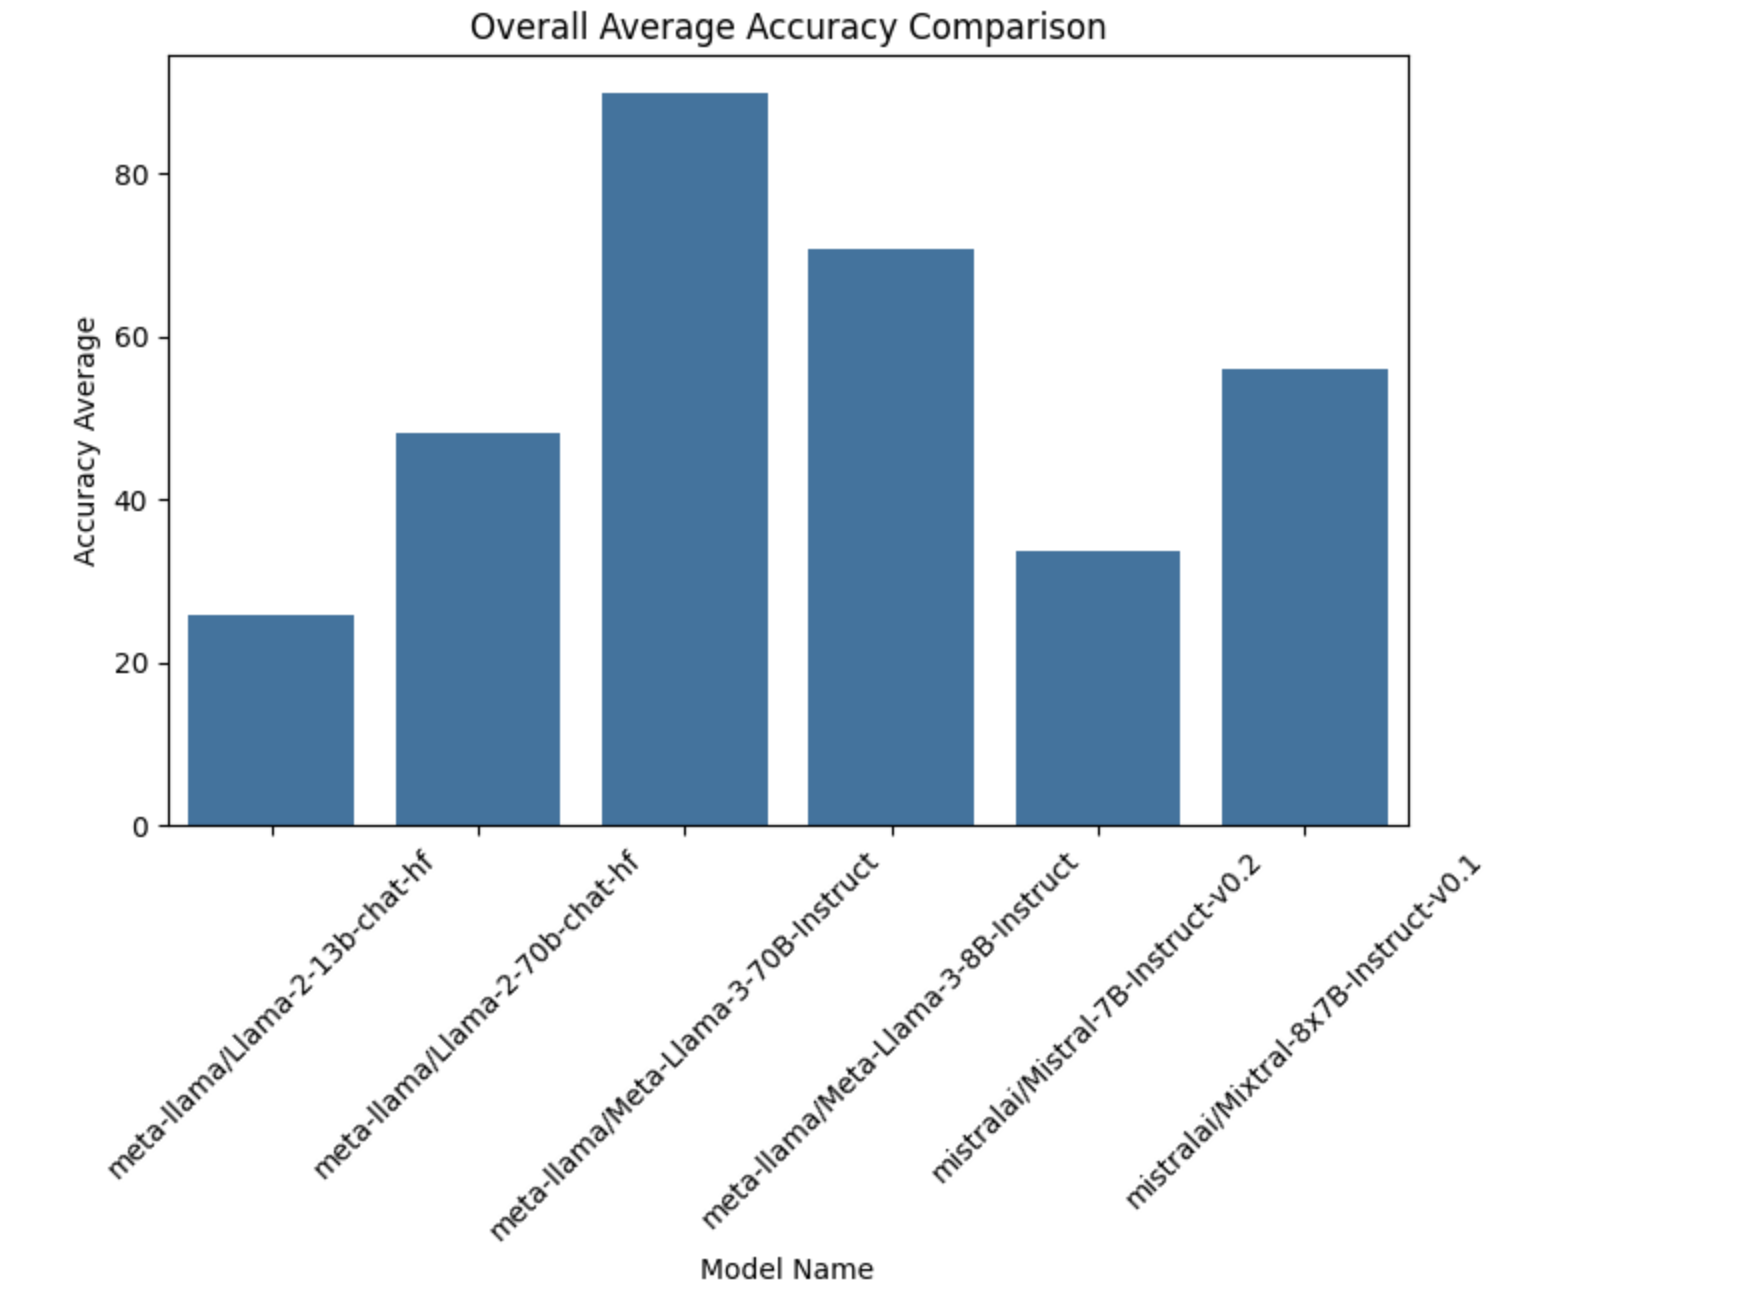
\includegraphics[width=\textwidth,]{report_template/images/bar_1.png}
    \caption{Bar plot comparing average accuracy of two sets of test data from GSM8K dataset across different language models.}
    \label{bar_1}
    \end{figure}

    \begin{figure}
    \centering
    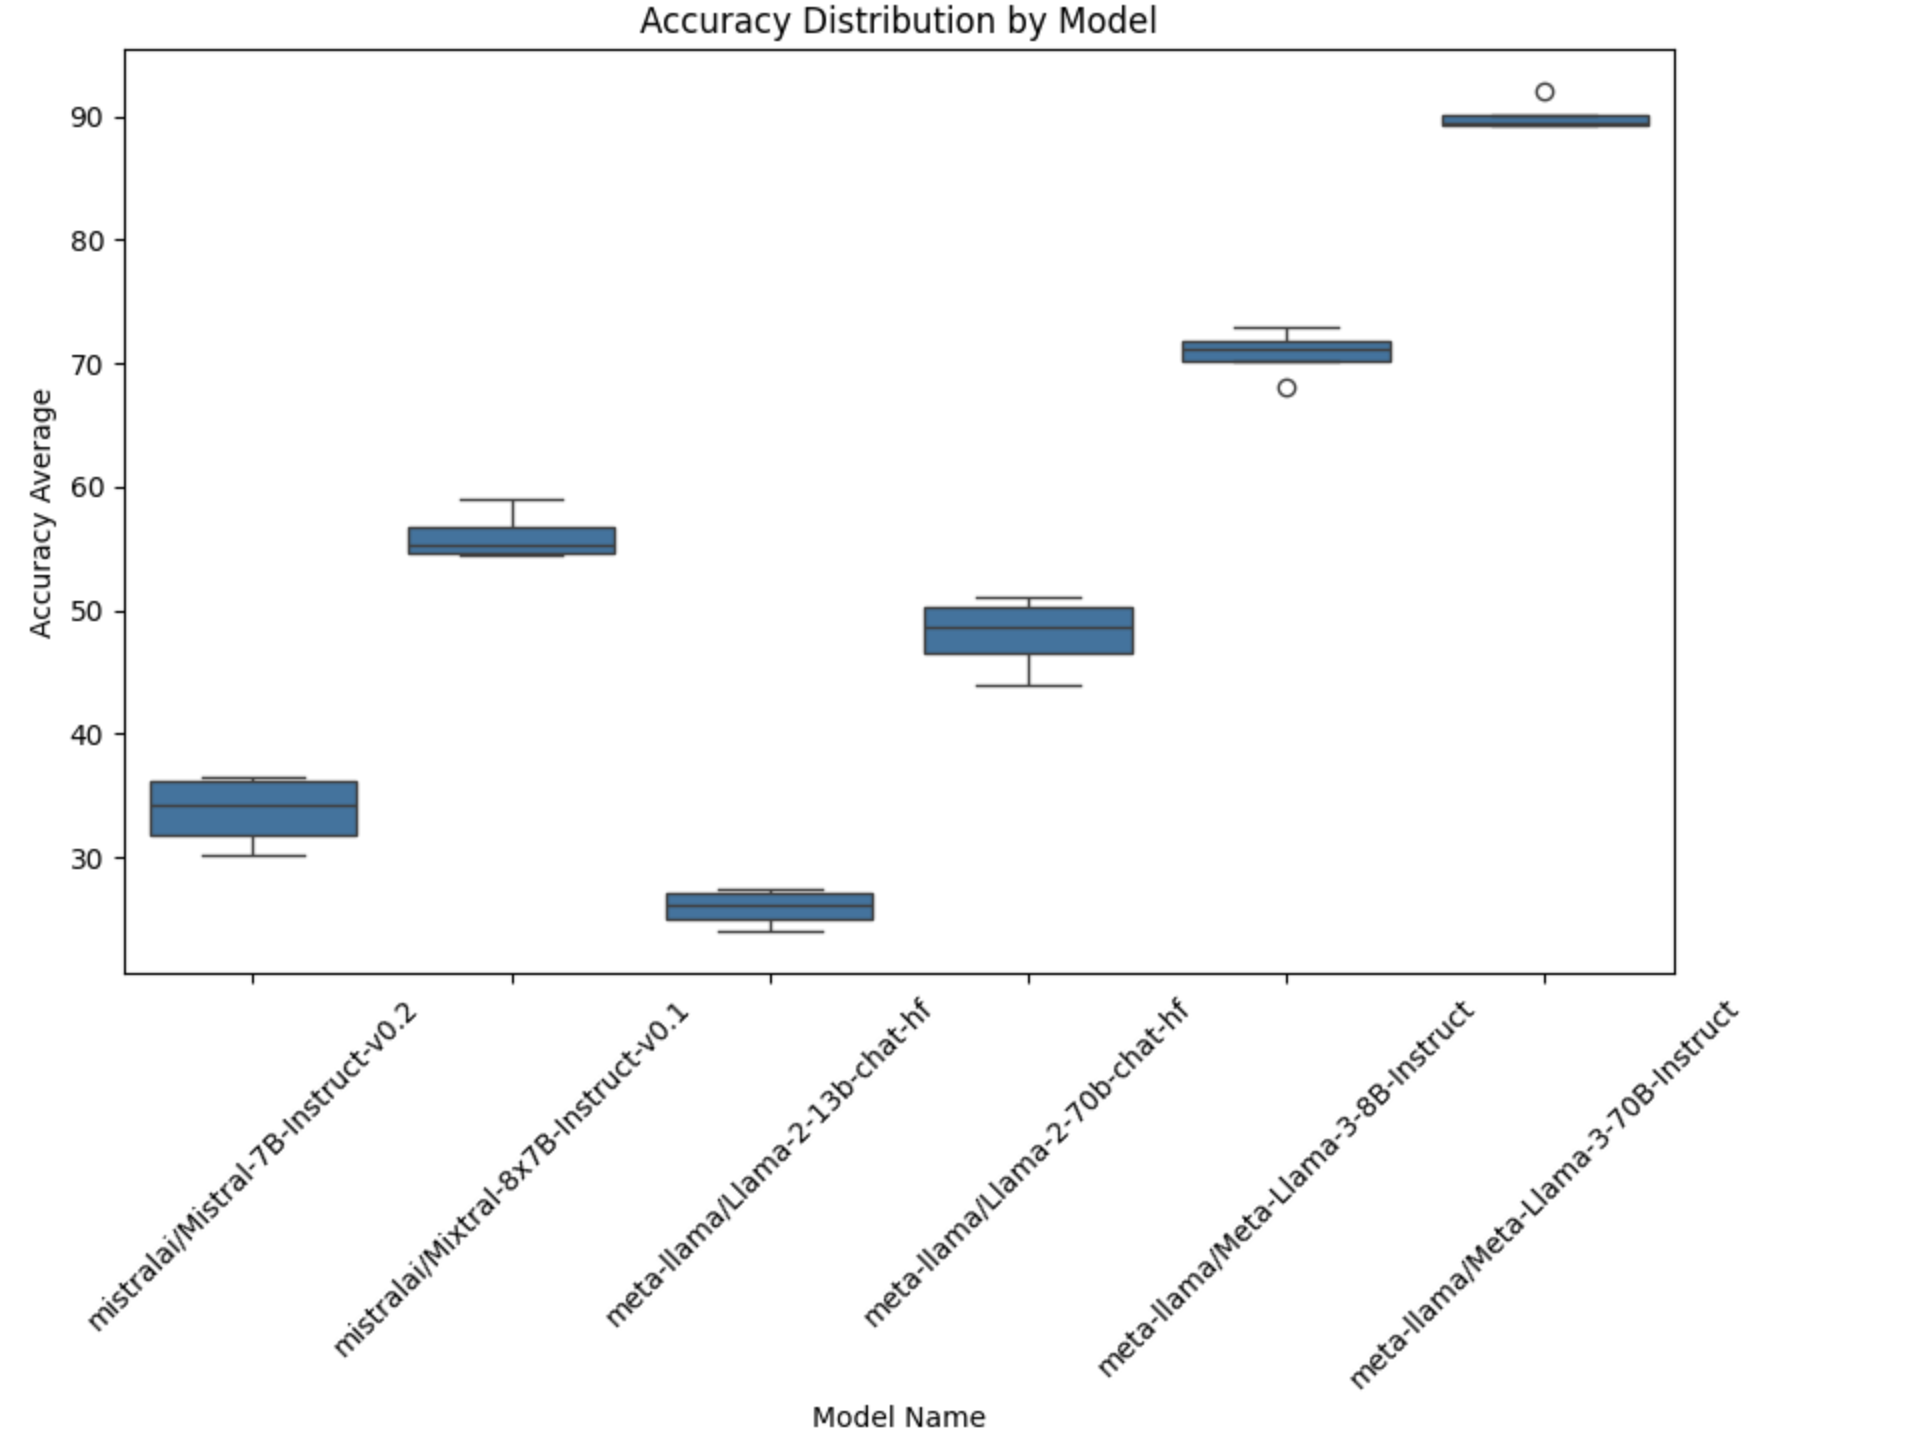
\includegraphics[width=\textwidth,]{report_template/images/box_1.png}
    \caption{Bar plot comparing average accuracy of two sets of test data from GSM8K dataset across different language models.}
    \label{box_1}
    \end{figure}

    \item \textbf{Sample Size Sensitivity Unveiled:} The utilization of DSPy's flexible evaluation pipeline allowed us to investigate the impact of test data sample size. The analysis showed a subtle but consistent decrease in accuracy as the sample size increased as shown in Figure \ref{line_1}, indicating potential challenges in model generalization and robustness to data variations.

    \begin{figure}
    \centering
    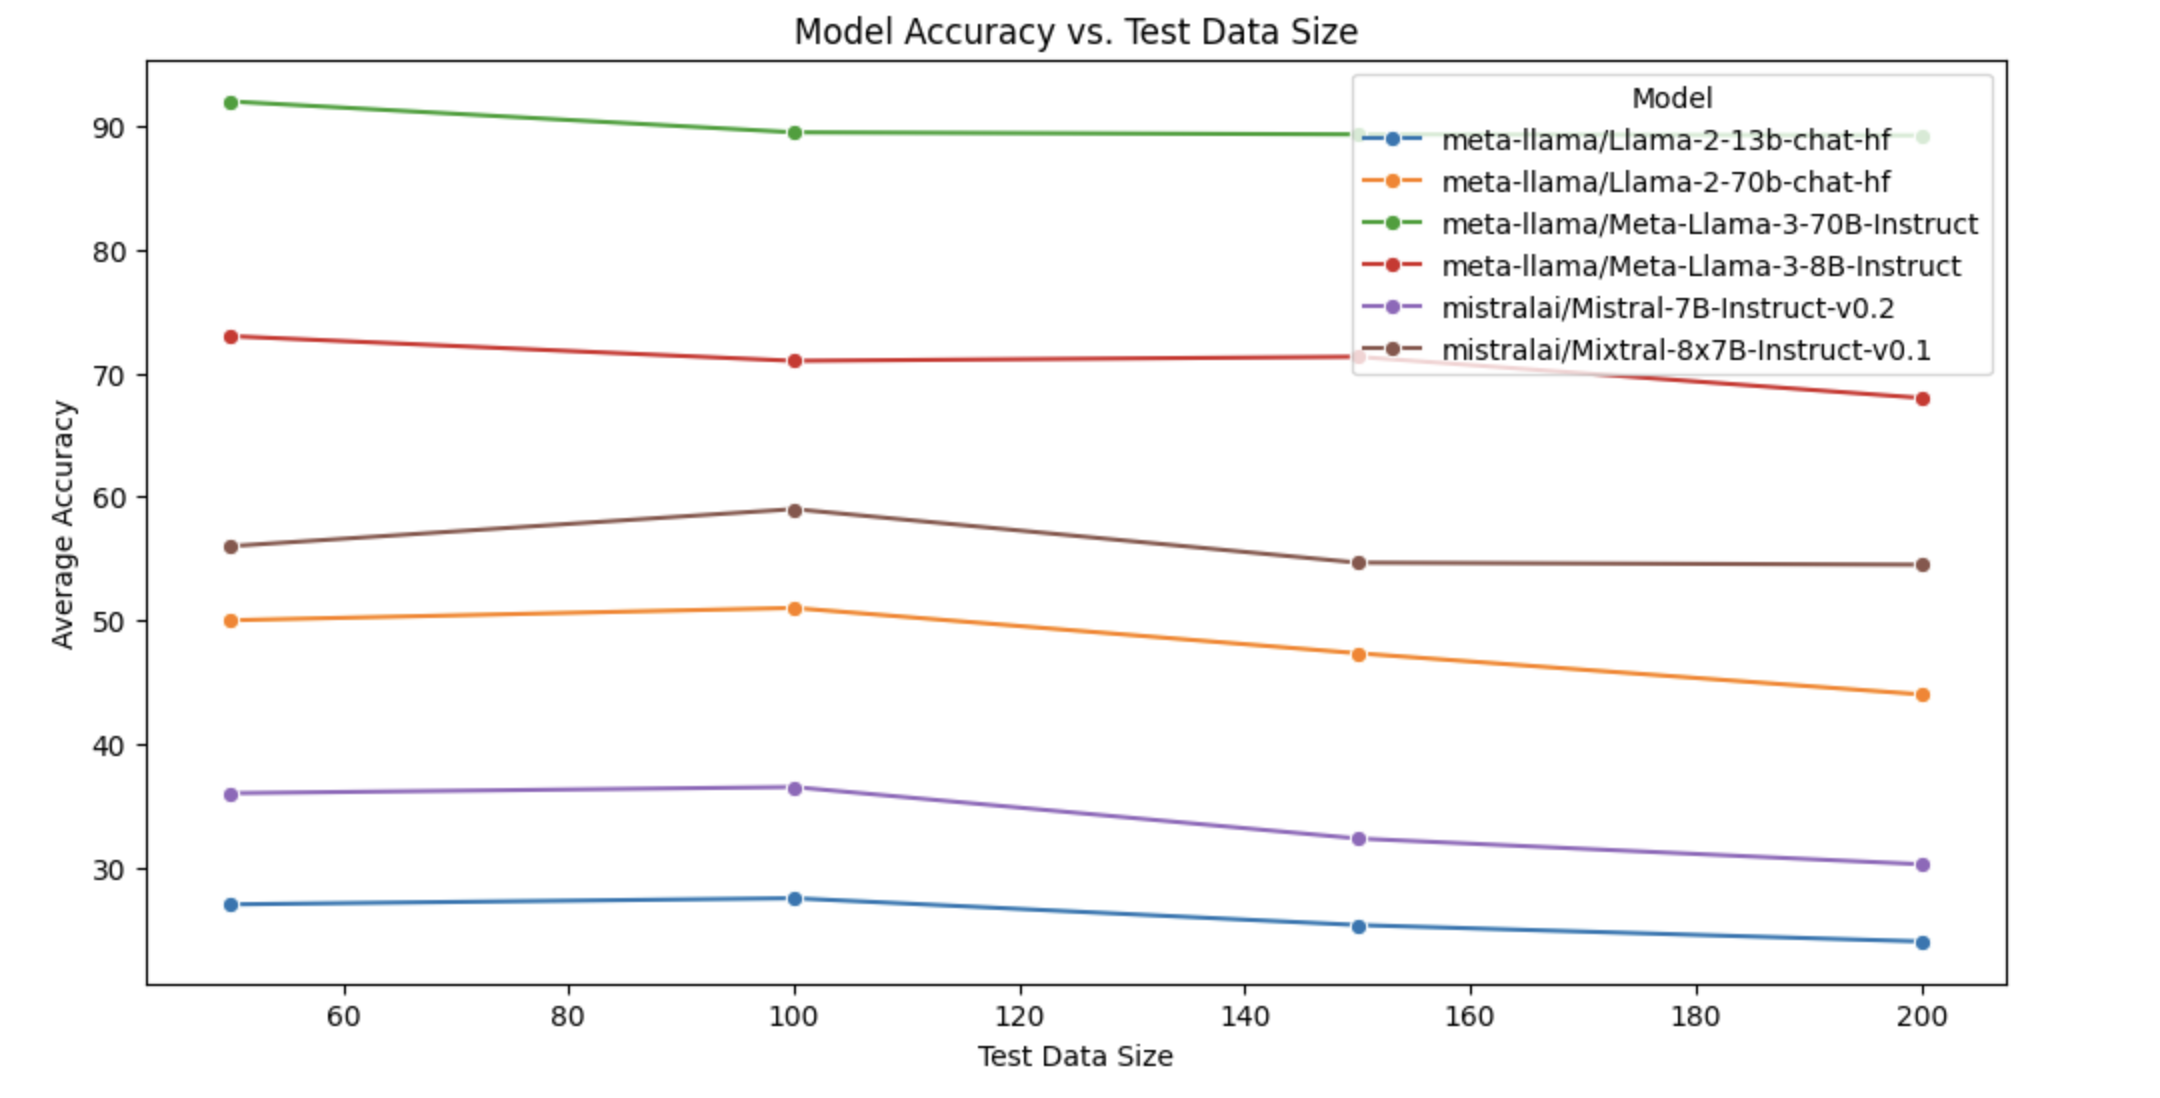
\includegraphics[width=\textwidth,]{report_template/images/line_1.png}
    \caption{Bar plot comparing average accuracy of two sets of test data from GSM8K dataset across different language models.}
    \label{line_1}
    \end{figure}

    \item \textbf{The Power of Instruction Fine-Tuning:} Through DSPy's comprehensive evaluation, we observed a clear advantage for models fine-tuned with instruction data. The inclusion of task-specific instructions during training, as facilitated by DSPy's seamless integration with various fine-tuning techniques, significantly enhanced model performance.

    \item \textbf{Accuracy Fluctuations Detected:} DSPy's fine-grained analysis revealed interesting fluctuations in model accuracy across different data samples, particularly for smaller models. This finding, made possible by DSPy's ability to conduct multiple evaluations and aggregate results, emphasizes the importance of robust evaluation strategies for accurately assessing LLM capabilities.
\end{enumerate}
\chapter{Requirements Resources}

\begin{enumerate}
    \item \textbf{Hardware:}
    \begin{itemize}
        \item For initial development and testing: Google Colab with GPUs (e.g., NVIDIA Tesla K80)
        \item For resource utilization studies and profiling: Linux virtual machine with:
            \begin{itemize}
                \item Minimum: 16 GB RAM, 6 vCPUs
                \item Recommended: 32 GB RAM, 8 vCPUs
            \end{itemize}
    \end{itemize}
    \item \textbf{Software:}
    \begin{itemize}
        \item Operating System: Linux for the virtual machine (recommended), macOS or Windows for initial development (optional)
        \item Programming Language: Python 3.8
        \item Libraries and Frameworks:
            \begin{itemize}
                \item DSPy (latest version)
                \item TensorFlow 2.x (latest version)
                \item Additional libraries for profiling (e.g., top, htop)
            \end{itemize}
    \end{itemize}
    \item \textbf{Datasets:}
    \begin{itemize}
    \item HotpotQA: Question answering dataset featuring natural, multi-hop questions, with strong supervision for supporting facts to enable more explainable question-answering systems.
    \item GSM8K: Consists of 8.5K high quality grade school math problems created by human problem writers.
    \end{itemize}
\end{enumerate}

\cleardoublepage
%\pagebreak
\phantomsection
\addcontentsline{toc}{chapter}{References}
\begin{singlespace}
\setlength\bibitemsep{8pt}
\printbibliography[title=References]
\end{singlespace}
\input{./appendix_a.tex}
\input{./appendix_b.tex}
%\backmatter % book mode only
\end{document}
